\documentclass[12pt]{article}
\usepackage{amsmath}
\usepackage{float}
\usepackage{amssymb}
\usepackage{graphicx}
\usepackage{hyperref}
\usepackage{cleveref}
\usepackage[most]{tcolorbox}
\usepackage[utf8]{inputenc}
\usepackage{tikz}
\usepackage{pstricks-add}
\usepackage{centernot}
\usepackage{enumerate}
\usepackage{MnSymbol}
\usepackage{mathtools}
\usepackage{subcaption}
\usepackage{geometry}
 \geometry{
 a4paper,
 total={170mm,257mm},
 left=20mm,
 top=20mm,
 }
\DeclarePairedDelimiter\ceil{\lceil}{\rceil}
\DeclarePairedDelimiter\floor{\lfloor}{\rfloor}
\DeclarePairedDelimiter\abs{\left|}{\right|}
\hypersetup{
    colorlinks=false,
    pdfborder={0 0 0},
}
\newcommand\tab[1][1cm]{\hspace*{#1}}
\newtheorem{theorem}{Theorem}
\newtheorem{corollary}{Corollary}
\usetikzlibrary{arrows,calc}
\title{MAT 1001: Calculus I}
\author{Alfonsus Rodriques Rendy}
\date{2021-10-21}

\begin{document}
\begin{center}
    \hspace*{-0.5cm}
    \framebox{
    \begin{minipage}{1\linewidth}
        \textbf{MAT1001 Calculus I} \\
        \vspace{-0.8cm}
        \begin{center}
            \huge{Lecture 12 - 15 : Integrals} 
            \\
            \vspace{0.5cm}
            \normalsize \textit{Lecture by Dr. Arjan Abeynaike} \\
            \vspace{0.3cm}
            \text{Scribe by Alfonsus Rodriques Rendy} \\
            \textrm{Oct 21, 2021 - Nov 2, 2021}
        \end{center}
    \end{minipage}}
\end{center}

\section{Antiderivatives}
\paragraph{Definition}
If $F'(x) = f(x)$ for all $x$ in an interval $I$, then $F$ is said to be an antiderivative of $f$ on $I$. 

\noindent
By corollary (2) of MVT, we have
\begin{theorem}[Antiderivative]
    If $F$ is an antiderivative of $f$ on an interval $I$, the the most general antiderivative of $f$ on $I$ is 
    \[
        F(x) + C
    \]
    where $C$ is an arbitrary constant.
\end{theorem}

\begin{figure}[h!]
     \centering
     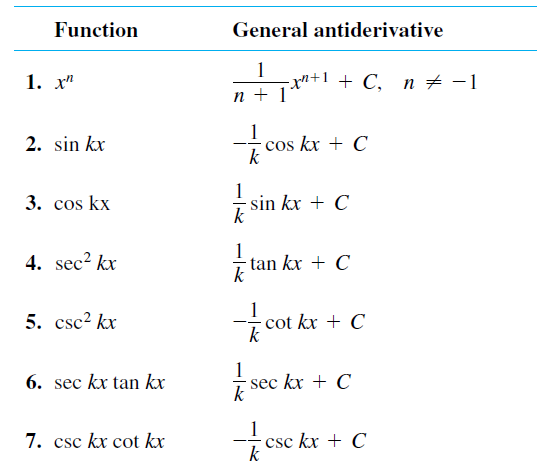
\includegraphics[width = 0.4\linewidth]{Images/general antiderivative.png}
     \caption{General antiderivative formula}
\end{figure}

\paragraph{Example 1} Find the antiderivative $F$ of $f(x) = 3 \sqrt{2} + \sin 2x$ that satisfies $F(0) = 1$!
\begin{align*} 
    f(x) &= 3 \sqrt{2} + \sin 2x \\
    F(x) &= 3(\frac{2}{3}) x^{\frac{3}{2}} - \frac{1}{2} \cos 2x + C \\
    F(0) &= 1 \Rightarrow 1 = - \frac{1}{2} + C \Rightarrow C = \frac{3}{2} \\
    F(x) &= 2 x^{\frac{3}{2}} - \frac{1}{2} \cos 2x + \frac{3}{2} \\
\end{align*}

\paragraph{Definition : Indefinite Integral}
The set of all antiderivatives of $f$ is called the \textbf{indefinite integrals} of $f$. 
If $F$ is one antiderivative of $f$, we write
\[
    \int f(x) \, dx = F(x) + C
\]
\noindent
$\int f(x) dx$ is called the indefinite integral of $f$ with respect to $x$ \\
$f(x)$ is the integrand. \\
$dx$ is called the variable of integration.

\paragraph{Example 1} Solve
\[
    \int (x^2 + x) dx
\]
\paragraph{Answer}
\begin{align*} 
    \int (x^2 + x) dx = \frac{1}{3}x^3 + \frac{1}{2}x^2 + C
\end{align*}
\paragraph{Example 2} Solve
\[
    \int (x^2 - 2x + 5) dx 
\]
\paragraph{Answer}
\[
    \int (x^2 - 2x + 5) dx =  \frac{1}{3}x^3 + x^2 + 5x +  C
\]

\paragraph{Note} Antiderivatives also apply linearity rule, that is
\[
    \int \alpha f(x) \pm \beta g(x) \, dx = \alpha \int f(x) \, dx \pm \beta \int g(x) \, dx
\]

\section{Finite Sums Estimations}
Consider finding the area $R$ under the graph of the function $y = 1-x^2$, above x-axis, between the vertical lines 
$x = 0$ and $x = 1$.

\begin{figure}[h!]
    \centering
    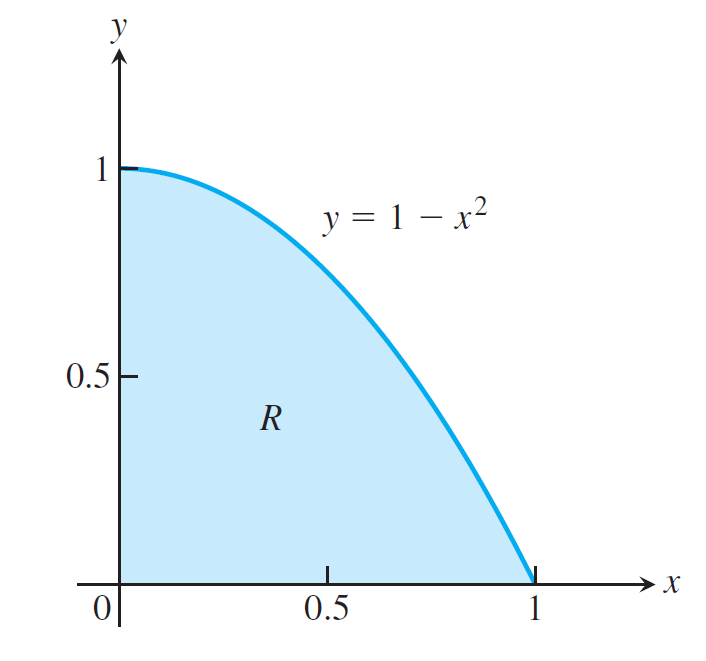
\includegraphics[width = 0.3\linewidth]{Images/area with summing.png}
\end{figure}

We may approximate $R$ by summing areas of rectangles with the following procedure: 
\begin{itemize} 
     \item Divide $[0,1]$ into sub-intervals with equal length and construct rectangles using the function values of the left/right endpoints.
     \item The sum areas the these rectangles is an approximation of $R$
\end{itemize}

First we divide $[a, b]$ into $n$ sub-intervals of the length $\Delta x = \frac{(b - a)}{n}$, that is 
with $[0, 1]$, $\Delta x = \frac{1}{n}$.
\subsection{Left Endpoint Sum}
Now, suppose we choose the left endpoint function value.
\begin{figure}[h!]
    \centering
    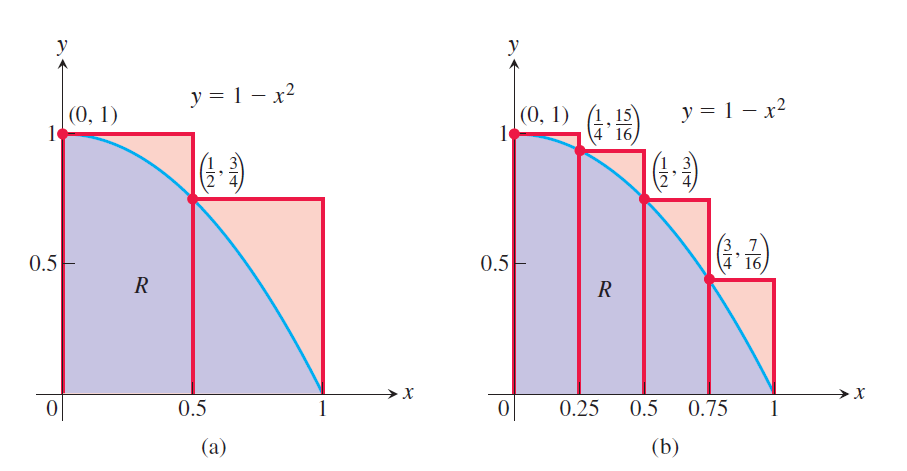
\includegraphics[width = 0.7\linewidth]{Images/left summing.png}
    \caption{(a) left endpoint sum, $n = 2$ (b) left endpoint sum, $n = 4$}
\end{figure}

\noindent
We have $x_1, x_2, ... x_n$, with $x_i$ as 
\[
    x_i = a + (i - 1)\frac{b - a}{n} 
\]
So, in the case of $[0, 1]$ with $n = 2$, $x_1 = 0$, $x_2 = 1/2$.
Hence,
\[
    Area = \frac{1}{2} \cdot \left(f(0) + f\left(\frac{1}{2}\right)\right) = \frac{1}{2} \left(1 + \frac{3}{4}\right) = \frac{7}{8}
\]
With $n = 4$, $x_1 = 0$, $x_2 = 1/4$, $x_3 = 1/2$, $x_4 = 7/16$.
Hence,
\[
    Area = \frac{1}{2} \cdot \left(f(0) + f\left(\frac{1}{4}\right) + f\left(\frac{1}{2}\right) + f\left(\frac{3}{4}\right)\right) = \frac{1}{2} \left(1 + \frac{15}{16} + \frac{3}{4} + \frac{7}{16}\right) = \frac{25}{32}
\]

\subsection{Right Endpoint Sum}
Instead of choosing the right endpoint function value, now suppose we choose the right endpoint function value.
\begin{figure}[h!]
    \centering
    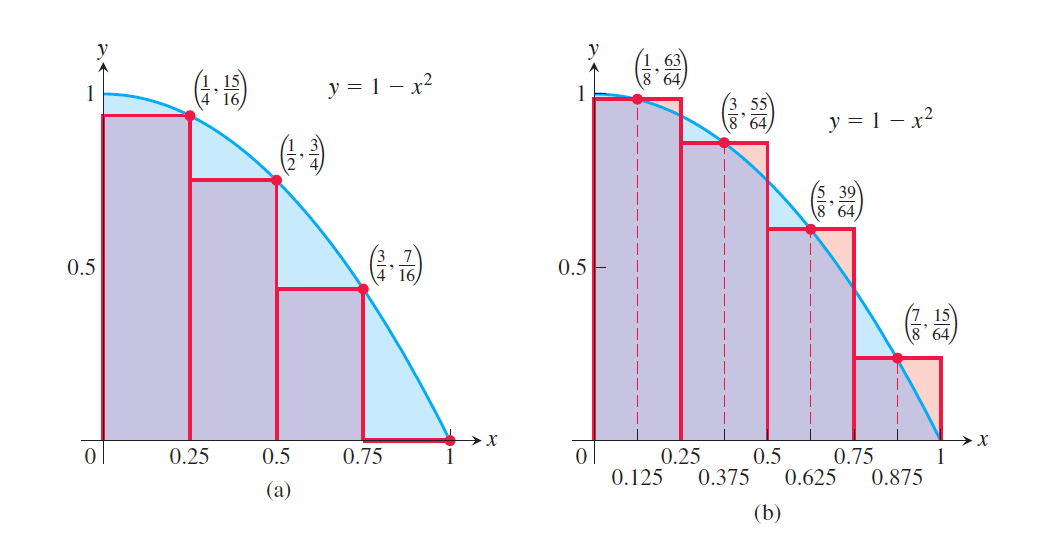
\includegraphics[width = 0.7\linewidth]{Images/right summing.png}
    \caption{(a) right endpoint sum, $n = 4$ (b) mid-point sum, $n = 4$}
\end{figure}

\noindent
We have $x_1, x_2, ... x_n$, with $x_i$ as 
\[
    x_i = a + i \left(\frac{b - a}{n} \right)
\]
So, in the case of $[0, 1]$ with $n = 4$, $x_1 = 1/4$, $x_2 = 1/2$, $x_3 = 3/4$, and $x_4 = 1$.
Hence,
\[
    Area = \frac{1}{4} \cdot \left(f\left(\frac{1}{4}\right) + f\left(\frac{1}{2}\right) + f\left(\frac{3}{4}\right) + f(1)\right) = \frac{1}{4} \left(\frac{15}{16} + \frac{3}{4} + \frac{7}{16} + 0 \right) = \frac{17}{32}
\]

\subsection{Area Approximation}
Let $n$ as the number of sub-intervals, then the length of the sub-intervals is $\Delta x = \frac{b - a}{n}$.We have 
$x_i = a + i(\Delta x) = a + i \left( \frac{b-a}{n} \right)$. The approximated area of $f(x)$ in the interval of $[a, b]$ is 
\[
    \frac{b - a}{n}\sum_{i = 1}^n f(c_i) 
\]
With $c_i \in [x_{i - 1}, x_i]$
\begin{itemize}
    \item For left endpoint sum, $c_i = x_{i - 1}$
    \item For right endpoint sum, $c_i = x_{i}$
    \item For mid point sum, $c_i = \frac{x_{i - 1} + x_{i}}{2}$
\end{itemize}

\subsection{Area Sums and Concavity}
Suppose $y = f(x)$ is \textbf{concave down} on $(a, b)$ and $f(x) \geq 0$, $\forall \, \in [a, b]$
\begin{itemize} 
    \item If we approximate the area between the curve and the x-axis, for $[a, b]$, using a midpoint sum $S$, 
    the sum will always over-estimate the area.
\end{itemize}

\noindent
Suppose $y = f(x)$ is \textbf{concave up} on $(a, b)$ and $f(x) \geq 0$, $\forall \, \in [a, b]$
\begin{itemize} 
    \item If we approximate the area between the curve and the x-axis, for $[a, b]$, using a midpoint sum  $S$, 
    the sum will always under-estimate the area.
\end{itemize}

\paragraph{Proof (Concave down - Midpoint)}
\begin{figure}[h!]
    \centering
    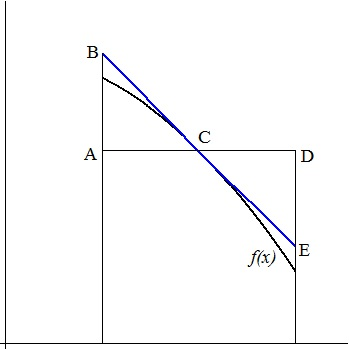
\includegraphics[width = 0.32\linewidth]{Images/overestimate concave down.jpg}
    \caption{$|AB| = |DE|$, so, $A_{sq} = A_{\triangle}$}
\end{figure}
The area under the tangent line = The area under the rectangle. Since on a concave down function, tangent line is always above the function, 
the area under the tangent line $>$ the area of the graph. So, the approximation will always over-estimate the area.
\subsection{Finite Sums}
Notation for finite sum is 
\[
    \sum_{i = 1}^n a_i = a_1 + a_2 + a_3 + \dots\, + a_n
\]
The variable $i$ is a "dummy variable" meaning it can be changed to a different symbol 
without changing the meaning.

\paragraph{Properties} Finite sums satisfy linearity, that is
\[
    \sum_{i = 1}^n (k \cdot a_i + t \cdot b_i) = k \sum_{i = 1}^n a_i + t \sum_{i = 1}^n b_i
\]

\noindent
There are some identities for specific finite sum, some of which are:
\[
    \sum_{i = 1}^n i = 1 + 2 + 3 + \dots + n = \frac{n}{2}(n + 1)
\]
\[
    \sum_{i = 1}^n i^2 = 1 + 4 + 9 + \dots + n^2 = \frac{n}{6}(n + 1)(2n + 1)
\]
\[
    \sum_{i = 1}^n i^3 = 1 + 8 + 27 + \dots + n^3 = \frac{n^2}{4}(n + 1)^2
\]

For $\sum_{i = 1}^n i^m$ we can find the formula by starting with $n^{m + 1}$ and using the formula for smaller $m$.

\paragraph{$m = 1$}  $\sum_{i = 1}^n i$ \\
Start with $n^2$, Let $S_n = \sum_{k = 1}^n k$
\[
    n^2 = (n^2 - (n - 1)^2) + ((n - 1)^2 - (n - 2)^2) + \dots\, + (2^2 - 1^2) + (1^2 - 0^2)
\]

Then we have
\begin{align*} 
    n^2 &= \sum_{k = 1}^n (k^2 - (k - 1)^2) \\
    &= \sum_{k = 1}^n (2k - 1) \\
    &= 2 \sum_{k = 1}^n k - n \\
    \sum_{k = 1}^n k &= \frac{n^2 + n}{2} \\
    S_n &= \frac{n}{2} (n + 1)
\end{align*}

\paragraph{$m = 2$}  $\sum_{i = 1}^n i^2$ \\
Start with $n^3$, Let $S_n = \sum_{k = 1}^n k^2$
\[
    n^3 = (n^3 - (n - 1)^3) + ((n - 1)^3 - (n - 2)^3) + \dots\, + (2^3 - 1^3) + (1^3 - 0^3)
\]

Then we have
\begin{align*} 
    n^3 &= \sum_{k = 1}^n (k^3 - (k - 1)^3) \\
    &= \sum_{k = 1}^n (k^3 - k^3 + 3k^2 - 3k + 1) \\
    &= \sum_{k = 1}^n (3k^2 - 3k + 1) \\
    &= 3 \sum_{k = 1}^n k^2 - 3 \sum_{k = 1}^n k + n \\
    &= 3 S_n - \frac{3n}{2} (n + 1) + n \\
    S_n &= \frac{1}{3}(n^3 + \frac{3n}{2} (n + 1) - n) \\
    S_n &= \frac{1}{6}(2n^3 + 3n^2 + n) \\
    S_n &= \frac{1}{6}(n)(n + 1)(2n + 1) \\
\end{align*}

\section{Riemann Sums}
\subsection{Definition}
\paragraph{Definition : Partition}
A partition of the interval $[a, b]$ is a set
\[
    P = {x_0, x_1, \dots, x_{n - 1}, x_n}
\]
such that 
\[
    a = x_0 < x_1 < \dots < x_{n - 1} < x_n = b 
\]

\paragraph{Definition : Riemann Sums}
Given a function $f:[a,b] \Rightarrow \mathbb{R}$ with a partition $P$ of $[a, b]$, a Riemann sum of
$f$ (w.r.t. $P$) is a sum of the form
\[
    S_P = \sum_{k = 1}^n f(c_k) \Delta x_k = f(c_1) \Delta x_1 + \dots\, + f(c_n) \Delta x_n
\]
where $c_k \in [x_{k - 1}, x_k]$ and $\Delta x_k = x_k - x_{k - 1}$ for each $k \in \{1, ..., n\}$

There are many Riemann sums for a function. It depends on the partition $P$ and the points $c$ chosen from the subintervals.
The left-endpoint, midpoint and right-endpoint sums are all special cases of Riemann sum.

\paragraph{Definition : Norm of Partition} Let $P = {x_0, x_1, x_2, ..., x_n}$ be a partition of $[a, b]$. The \textbf{norm} of $P$ denoted by $||P||$ is defined by
\[
    || P || = \max_{k: 1 \leq k \leq n} \Delta x_n
\]
That is, $||P||$ is the length of the largest subinterval given by $P$.

\paragraph{Example}
The partition of $P = [0, 2]$ represented below has norm $||P|| = 0.5$
\begin{figure}[h!]
     \centering
     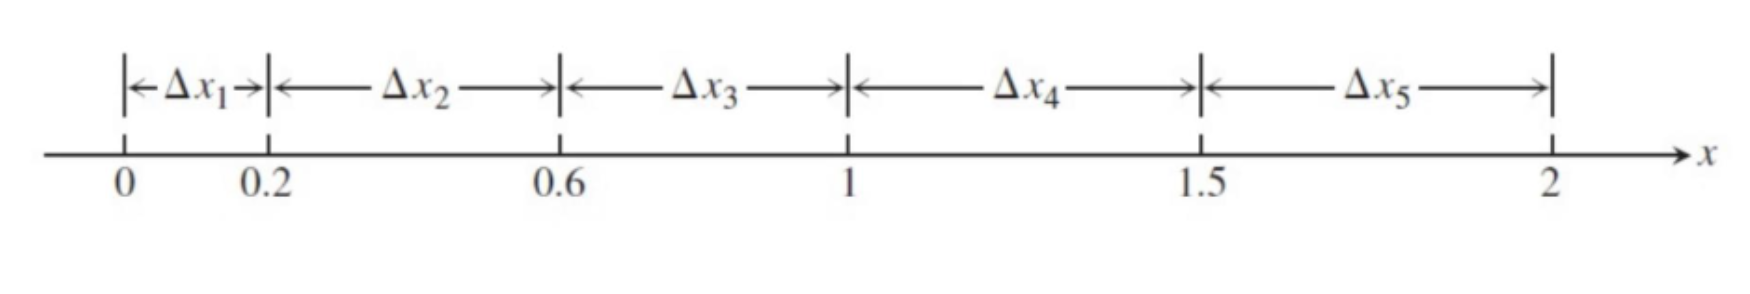
\includegraphics[width = 0.9\linewidth]{Images/norm.png}
\end{figure}

\section{Definite Integrals}
\subsection{Definition}
Let $f(x)$ be a function defined on a closed interval $[a, b]$ . We say
that a number $J$ is the definite integral of $f$ over $[a, b]$ and that $J$ is the limit of
the Riemann sums $\sum_{k = 1}^n f(c_k) \Delta x_k$ if the following condition is satisfied:

Given any number $\epsilon > 0$ there is a corresponding number $\delta > 0$ such that
for every partition $P = {x_0, x_1, ... , x_n}$ of $[a, b]$ with $||P|| < \delta $ and any choice
of $c_k$ in $[x_{k-1}, x_k]$, we have
\[
    \left|\sum_{k = 1}^n f(c_k) \Delta x_k - J \right| < \epsilon
\]
By definition, we can write the above definition as
\[
    \lim_{||P|| \to 0} \sum_{k = 1}^n f(c_k) \Delta x_k = J
\]
If the limit $J$ exists, we say that $f$ is integrable on $[a, b]$ and write the
limit $J$ as 
\[
    \int_{a}^{b} f(x) dx  
\]
It's called the \textbf{definite integral} or Riemann integral of $f$ over $[a, b]$
\subsection{Integrability}
\begin{theorem}[Integrability of Continuous Functions]
    If a function $f$ is continuous over the interval $[a, b]$ , or if $f$ has at most finitely many jump or removable discontinuities
    there, then the definite integral $\int_a^b f(x) \, dx$ exists and $f$ is integrable over $[a, b]$
\end{theorem}

\paragraph{Proof}
For each $[x_{k - 1}, x_k]$ we define:
\begin{itemize} 
    \item $M_k = \max\{f_{x_k^*} : x_k^* \in [x_{k - 1}, x_k]\}$
    \item $m_k = \min\{f_{x_k^*} : x_k^* \in [x_{k - 1}, x_k]\}$
\end{itemize}
Or we say $M_k$ as the maximum value of $f(c)$ with $c \in [x_{k - 1}, x_k]$ and
$m_k$ as the minimum value of $f(c)$ with $c \in [x_{k - 1}, x_k]$

From that, we have
\begin{align*} 
    U_p(f) = \sum_{k = 1}^n M_k \Delta x_k \textrm{\tab Upper sum}\\
    L_p(f) = \sum_{k = 1}^n m_k \Delta x_k \textrm{\tab Lower sum}
\end{align*}

Thus for each $c_k \in [x_{k - 1}, x_k]$, $m_k \leq f(c_k) \leq M_k$, So
\[
    L_p = \sum_{k = 1}^n m_k \Delta x_k \leq \sum_{k = 1}^n f(c_k) \Delta x_k \leq \sum_{k = 1}^n M_k \Delta x_k = U_p
\]
As $||P|| \to 0$, $U_p - L_p \to 0$. Or, for any given $\epsilon$, choose all 
$\Delta x_k $ small enough such that $M_k - m_k < \frac{\epsilon}{b - a}, \forall \, k$. Then,
\[
    U_p(f) - L_p(f) = \sum_{k = 1}^n (M_k - m_k) \Delta x_k < \frac{\epsilon}{b - a} \sum_{k - 1}^n \Delta x_k
\]
Since
\[
    \frac{\epsilon}{b - a} \sum_{k - 1}^n \Delta x_k = \frac{\epsilon}{b - a}(b - a) = \epsilon
\]
We have
\[
    U_p(f) - L_p(f) < \epsilon    
\]
Hence
\begin{align*} 
     \lim_{||P|| \to 0} (U_p(f) - L_p(f)) &= 0 \\
     \lim_{||P|| \to 0} U_p(f) &= \lim_{||P|| \to 0} L_p(f))  \\
\end{align*}

\noindent
Since all Riemann sums $S_p = S_p(f)$ satisfy
\[
    L_p(f) \leq S_p(f) \leq U_p(f)
\]
then
\[
    \lim_{||P|| \to 0} S_p(f) = \lim_{||P|| \to 0} \sum_{k = 1}^n f(c_k)\Delta x_k
\]
must exists.

\subsection{Computation Riemann Integrals}
Suppose we know that $f$ is integrable on $[a, b]$. Then we can compute the limit of Riemann sums by choosing any sequence of partitions
$P$ such that $||P|| \to 0$.

In particular, we may choose $\Delta x_k = \Delta x = \frac{b - a}{n}$ or $P$ divides
$[a, b]$ into $n$ subintervals of equal length.

Then we can compute the definite integral as:
\[
    \int_a^b f(x) \, dx = \lim_{n \to \infty} \sum_{k = 1}^n f(c_k) \Delta x
\]
With $c_k \in [x_{k-1}, x_k]$ can be chosen in any way.

\paragraph{Example} Evaluate $\int_0^1 x^2 dx$ using Riemann sums.

\begin{align*} 
    \int_0^1 x^2 dx &= \lim_{n \to \infty} \sum_{k = 1}^n x_k^2 \Delta x = \lim_{n \to \infty} \sum_{k = 1}^n \left(\frac{x}{k}\right)^2 \cdot \frac{1}{n} \\
    &= \lim_{n \to \infty} \frac{1}{n^3} \sum_{k = 1}^n k^2 \\
    &= \lim_{n \to \infty} \frac{1}{n^3}(\frac{1}{6}n(n + 1)(2n + 1)) \\
    &= \frac{1}{3}
\end{align*}
Choosing the right endpoint as $c_k$ gives the similar result.

\subsection{Nonintegrability}
$\int_a^b f(x) dx$ does not exist when the upper sum and the lower sum do not converge to the 
same number $J$. In other words, here exists $\epsilon > 0$ such that no matter how small a given $\delta > 0$ is, 
there is a partition $P$ of $[a, b]$ with $||P|| < \delta$ such that $U_p(f) - L_p(f) > \epsilon$. $\epsilon$ is gap 
between $L_p(f)$ and $U_p(f)$.

\paragraph{Example} Dirichlet function
\begin{align*} 
     f(x) = 
     \begin{cases} 
        1 \textrm{\tab if } x \in \mathbb{Q} \\
        0 \textrm{\tab if } x \notin \mathbb{Q} \\
     \end{cases} 
\end{align*}

Then $\int_a^b f(x) dx$ does not exist for all $a, b$ with $a < b$.

\paragraph{Proof}
For any interval $[x_{k-1}, x_k]$ we have some values 
$c_1, c_2 \in [x_{k -1}, x_k]$ such that $f(c_1) = 1$ and $f(c_2) = 0$.
hen for any partition $P$ of $[a, b]$ with $||P|| < \delta$,
\begin{align*} 
     L_p = \sum_{k = 1}^n m_k \, \Delta x_k = \sum_{k = 1}^n 0 \, \Delta x_k = 0 \\
     U_p = \sum_{k = 1}^n M_k \, \Delta x_k = \sum_{k = 1}^n 1 \, \Delta x_k = b - a
\end{align*}
Hence, 
\[
    U_p(f) - L_p(f) = b - a > \epsilon
\]
and integral does not exists
\section{Properties of Integral}
\paragraph{Definition}
For $a < b$ we define:
\[
    \int_{a}^{b} f(x) dx = - \int_{a}^{b} f(x) dx
\]

\[
    \int_{a}^{a} f(x) dx = 0
\]
Other rules of integral:
\begin{figure}[H]
    \centering
    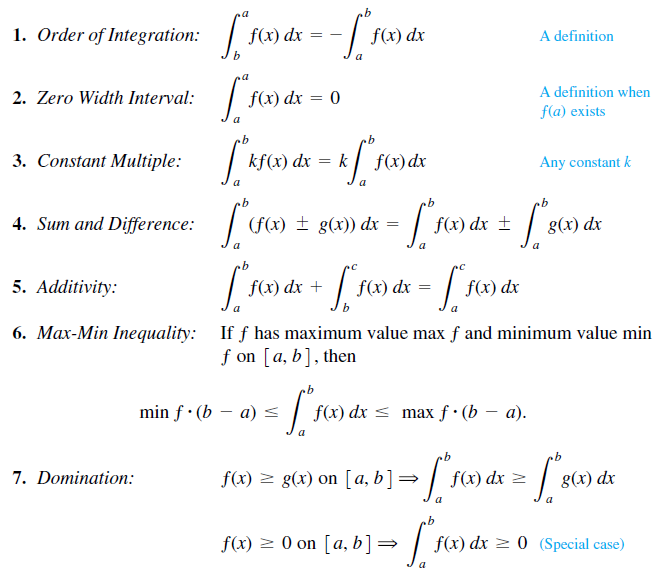
\includegraphics[width = 0.6\linewidth]{Images/rules of integrals.png}
    \caption{Other rules of definite integrals}
\end{figure}

\begin{figure}[H]
    \centering
    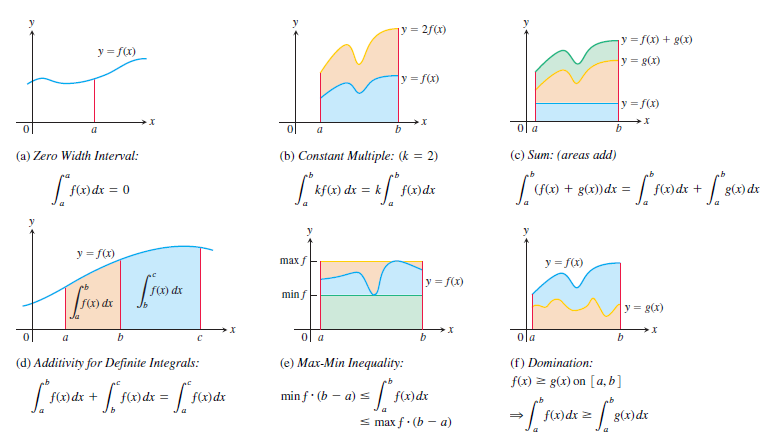
\includegraphics[width = 1\linewidth]{Images/rules of integrals 2.png}
    \caption{Geometric Illustration of rules of definite integrals}
\end{figure}

\paragraph{Note} Additivity (property 5) works for $b \in [a, c]$ even if $b \notin [a, c]$. For example:
\[
    \int_{3}^{5} f(x) dx + \int_{5}^{6} f(x) dx = \int_{3}^{6} f(x) dx
\]
then
\[
    \int_{3}^{5} f(x) dx = \int_{3}^{6} f(x) dx - \int_{5}^{6} f(x) dx
\]
\[
    \int_{3}^{5} f(x) dx = \int_{3}^{6} f(x) dx + \int_{6}^{5} f(x) dx
\]

\paragraph{Note} All properties (3-6 and 7(i)) work even if there exists  $f < 0$ on $[a, b]$ 
and even if $f$ is not continuous

\paragraph{Proof of Property 6}
Suppose $\int_{a}^{b} f(x) dx$ exists. Let 
\[
  M = \max_{x \in [a, b]} f(x) \textrm{\tab and \tab} m = \min_{x \in [a, b]} f(x)
\]
Then every Riemann sum satisties
\[
    m \sum_{k = 1}^n \Delta x_n = \sum_{k = 1}^n m \Delta x_n \leq \sum_{k = 1}^n f(c_k) \Delta x_n \leq \sum_{k = 1}^n M \Delta x_n = M \sum_{k = 1}^n \Delta x_n
\]
So,
\[
    m \lim_{ \mid \mid P \mid \mid \to 0} \sum_{k = 1}^n \Delta x_n \leq \lim_{ \mid \mid P \mid \mid \to 0} \sum_{k = 1}^n f(c_k) \Delta x_n \leq M \lim_{ \mid \mid P \mid \mid \to 0} \sum_{k = 1}^n \Delta x_n
\]
Hence
\[
    m \int_{a}^{b} dx \leq \int_{a}^{b} f(x) dx \leq M \int_{a}^{b} dx  
\]
Note that  $\int_{a}^{b} dx = b - a$
Then:
\[
    m(b - a) \leq \int_{a}^{b} f(x) dx \leq M(b - a)
\]

\paragraph{Example} Since $0 \leq \sqrt{1 + \cos x} \leq \sqrt{2}$ for all $x$, by domination:
\[
    \int_{0}^{1} 0 \, dx \leq \int_{0}^{1} \sqrt{1 + \cos x} \, dx \leq  \int_{a}^{b} \sqrt{2} \, dx 
\]
Hence
\[
    0 \leq  \int_{0}^{1} \sqrt{1 +  \cos x} \, dx \leq \sqrt{2}
\]

\section{Average Value of Function}
Let $v(t)$ be the velocity of an object at time $t$, where $v(t) \geq 0$ for all $t \in [a, b]$ \\
Then $\sum_{k = 1}^n v(c_k) \Delta t_k$ is an approximated distance travelled over time interval $[a,b]$ \\
$\int_{a}^{b} v(t)$ is the total distance travelled over $[a, b]$

Hence: $\frac{1}{b - a} \int_a^b v(t) dt$ is average velocity

\paragraph{Definition}
If $f$ is integrable on $[a, b]$, then its average value on $[a, b]$, also called its mean, is 
\[
    av(f) = \frac{1}{b - a} \int_a^b f(x) dx 
\]
\paragraph{Example} What is the average value of $f(x) = \sqrt{4 - x^2}$ with $x \in [-2, 2]$
\begin{figure}[H]
    \centering
    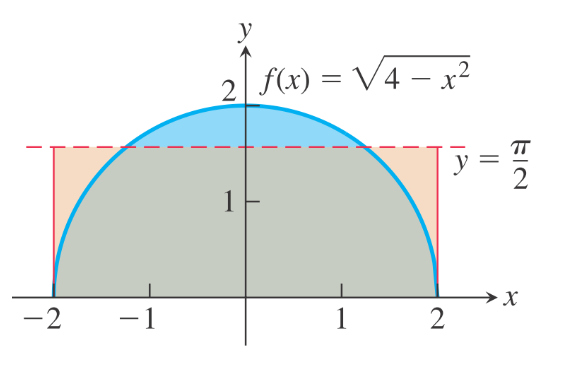
\includegraphics[width = 0.5\linewidth]{Images/average example.png}
\end{figure}
\paragraph{Answer}
\begin{align*} 
     av(f) &= \frac{1}{2 - ( - 2)} \int_{ - 2}^2 \sqrt{4 - x^2} dx \\
     &= \frac{1}{4} \cdot \frac{1}{2} \pi (2)^2 \\
     &= \frac{\pi}{2}
\end{align*}

\section{MVT of Definite Integrals}
\begin{theorem}[MVT for Definite Integrals]
     If $f$ is continuous on $[a, b]$ then at some point $c \in [a, b]$
     \[
         f(c) = \frac{1}{b - a} \int_a^b f(x) dx
     \]
\end{theorem}

\paragraph{Geometric Representation}
If $f$ is continuous, then there is a point $c \in [a, b]$ such that $f(c)$ is the average height
\begin{figure}[H]
     \centering
     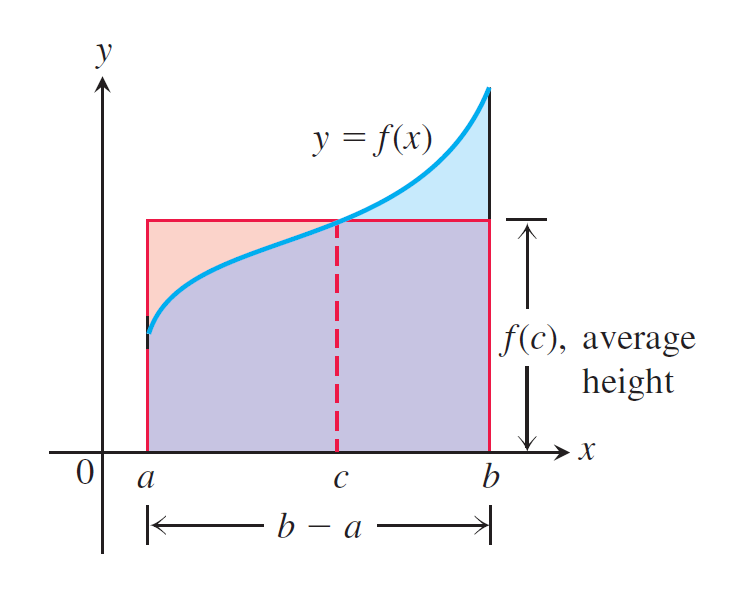
\includegraphics[width = 0.5\linewidth]{Images/mvt integral.png}
     \caption{$f(c)$ is the average height of $f$ on $[a, b]$}
\end{figure}

\paragraph{Proof}
Since $f$ is continuous, there exist $x_1$ and $x_2$ in $[a, b]$ such that 
\[
    f(x_1) = m = \min_{x \in [a, b]} f(x) \textrm{\tab and \tab} f(x_2) = M = \max_{x \in [a, b]} f(x)
\]
Let assume that $x_1 \neq x_2$. By min-max inequality, we have
\[
    m(b - a) \leq \int_a^b f(x) dx \leq M(b - a)
\]
By IVT
\[
    f(c) = \frac{1}{b - a} \int_a^b f(x) dx 
\]
for some $c$ between $x_1$ and $x_2$. So, $c \in [a, b]$

\paragraph{Note} The condition of the theorem applies is \textbf{continuity}.
\paragraph{Example}
\begin{figure}[H]
    \centering
    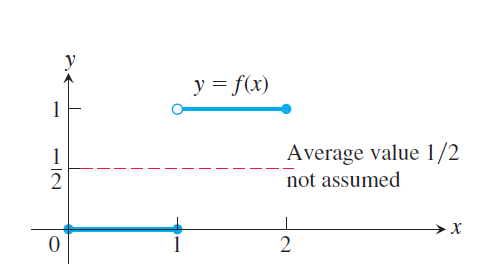
\includegraphics[width = 0.4\linewidth]{Images/mvt discontinuous.png}
\end{figure}

Since $f(x)$ is not continuous at $x = 1$:
\[
    \int_0^2 f(x) dx = \int_0^1 f(x) dx + \int_1^2 f(x) dx = 0 + 1 = 1
\]
Hence, 
\[
    av(f) = \frac{1}{2}
\]
However, the average value is not equal to the function at any point on $[0, 2]$. So, \textbf{the average value need not to be assumed}.

\paragraph{Consequence} If $f$ is continuous on $[a, b]$, $a \neq b$ and if $\int_a^b f(x) dx = 0$ then $f(x) = 0$ at least once in $[a, b]$

\section{The Fundamental Theorem of Calculus}
\subsection{FTC Part 1}
\paragraph{Intuition}
Let $v(t)$ be the velocity of an object at time $t$, where $v(t) \geq 0$ for all $t = [1,8]$. Then:
\begin{itemize} 
    \item $\int_1^5 v(t) dt$ represent the distance travelled from $t = 1$ to $t = 5$
    \item If $F(t) = \int_1^x v(t)$ then $F(x)$ represent the distance travelled between $t = 1$ and $t = x$
    \item Then $F'(x)$ is the instantenous velocity at $t = x$
\end{itemize}
\begin{theorem}[The Fundamental Theorem of Calculus Part 1]
    If $f$ is continuous on $[a, b]$ then $F(x) = \int_a^x f(t) dt$ is continuous on $[a, b]$ and differentiable on $(a, b)$ and its derivative is $f(x)$
    \[
        F'(x) = \frac{d}{dx} \int_a^x f(t) dt = f(x)
    \]
\end{theorem}
\begin{figure} 
    \centering
    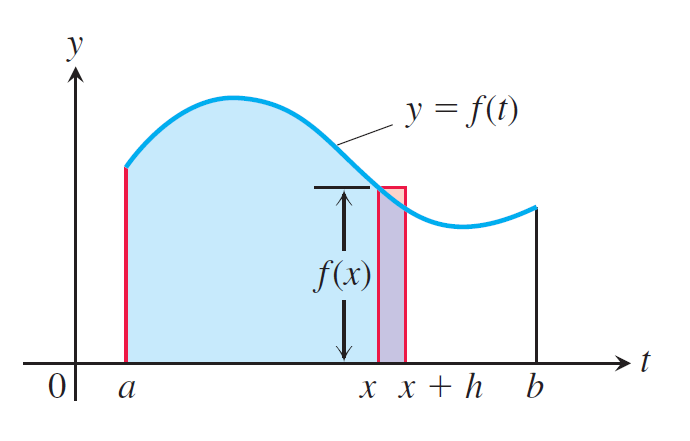
\includegraphics[width = 0.4\linewidth]{Images/ftc 1.png}
    \caption{Illustration of FTC 1}
\end{figure}
\paragraph{Proof FTC Part 1}
Suppose $f$ is continuous on $[a, b]$. Let $F : [a, b] \to \mathbb{R}$, $F(x) = \int_a^x f(t)\: dt$
\begin{align*} 
     F'(x) &= \lim_{h \to 0} \frac{F(x + h) - F(x)}{h} \\ 
     &= \lim_{h \to 0} \frac{\int_a^{x + h} f(t)\:  dt - \int_a^{x} f(t)\: dt }{h} \\ 
     &= \lim_{h \to 0} \frac{\int_a^{x + h} f(t)\: dt + \int_x^{a} f(t)\: dt }{h} \\ 
     &= \lim_{h \to 0} \frac{\int_x^{x + h} f(t)\: dt}{h} \\ 
\end{align*}
\noindent
For $h > 0$, by MVT for integrals, 
\[
    \frac{1}{h} \int_x^{x + h} f(t) dt = f(c)
\]
for some $c \in [x, x + h]$
As $h \to 0^{+}$, $c \to x^{+}$, so
\[
    F^{'}_{+} (x) = \lim_{h \to 0^{+}} f(c) = \lim_{c \to x^{+}} f(c) = f(x)
\]
\noindent
For $h < 0$, by MVT for integrals, 
\[
    \frac{1}{h} \int_x^{x + h} f(t) dt =  \frac{1}{ - h} \int_x^{x + h} f(t) dt = f(c)
\]
for some $c \in [x + h, x]$
As $h \to 0^{-}$, $c \to x^{-}$, so
\[
    F^{'}_{-} (x) = \lim_{h \to 0^{-}} f(c) = \lim_{c \to x^{-}} f(c) = f(x)
\]
Hence, 
\[
    F'(x) = f(x)\qquad \forall\: x \in (a,b)
\]
\noindent

\paragraph{Remark} We have showed that
\[
    F'(x) = f(x)\qquad \forall\: x \in (a,b)
\]
Hence, $F$ is differentiable on interval $(a, b)$ and continuous on interval $(a, b)$. The same argument can also be used to show That
\[
    F^{'}_{ + }(a) = f(a) \textrm{\tab and \tab} F^{'}_{- }(b) = f(b)
\]
Hence, $F$ is one-sided differentiable at $x = a$ and $x = b$. Therefore, $F$ is continuous on $[a, b]$.

\paragraph{Example 1} $y = \int_a^x (t^3 + 1)\: dt$ \\
Let $F(x) = y = \int_a^x (t^3 + 1)\: dt$ and $f(t) = t^3 + 1$
By FTC 1, 
\[
    \frac{dy}{dx} = F'(x) = f(x) = x^3 + 1 
\]

\paragraph{Example 2} $y = \int_x^5 (3t \sin t)\: dt$ \\
Let $F(x) = y = \int_5^x (3t \sin t)\: dt$ and $f(t) = 3t \sin t$.  \\
By FTC 1, 
\[
    \frac{dy}{dx} = - F'(x) = - f (x) = - 3x \sin x
\]

\paragraph{Example 3} $y = \int_1^{x^2} (\cos t)\: dt$ \\
Let $F(x) = y = \int_1^u (\cos t)\: dt$ and $u = x^2$. So, $y = F(u)$ \\
By FTC 1, 
\[
    \frac{dy}{du} = F'(u) = \cos u = \cos (x^2)
\]
By chain rule,
\[
    \frac{dy}{dx} = \frac{dy}{du} \frac{du}{dx} = 2x \cos (x^2)
\]

\paragraph{Example 4} $y = \int_{1 + 3x^2}^{4} (\frac{1}{2 + t})\: dt$ \\
Let $F(x) = y = \int_4^u (\cos t)\: dt$ and $u = 1 + 3x^2$. So, $y = - F(u)$ \\
By FTC 1, 
\[
    \frac{dy}{du} = - F'(u) = - \frac{1}{2 + u} = - \frac{1}{3 + 3x^2}
\]
By chain rule,
\[
    \frac{dy}{dx} = \frac{dy}{du} \frac{du}{dx} = - \frac{6x}{3 + 3x^2} = - \frac{2x}{1 + x^2}
\]

\paragraph{Remark} If $F(u) = \int_a^u f(t)\:  dt$ then
\[
    \int_a^{g(x)} f(t)\: dt = (F \circ g)(x) = F(g(x))
\]
By chain rule,
\[
    \frac{d}{dx} \int_a^{g(x)} f(t)\: dt = (F \circ g)(x) = F'(g(x))g'(x) 
\]
By FTC 1,
\[
    F'(g(x))g'(x)  = f(g(x))g'(x) 
\]
Hence,
\[
    \frac{d}{dx} \int_a^{g(x)} f(t)\: dt = f(g(x))g'(x) 
\]
\subsection{FTC Part 2}
\begin{theorem} 
    If $f$ is continuous over $[a, b]$ and $F$ is any antiderivative of $f$ on $[a, b]$, Then
    \[
        \int_a^b f(x) \, dx = F(b) - F(a)
    \]
\end{theorem}
\paragraph{Proof FTC Part 2}
Let $G(x) = \int_a^x f(t) dt$. By FTC 1, $G$ is an antiderivative of $f$ on $(a, b)$. Since $F$ is also an antiderivative of $f$, 
$\exists \: c$ such that 
\[
    G(x) = F(x) + c\qquad\: \forall \: x \in (a, b)
\]
$G$ and $F$ are continuous at a, since
\[
    G(a) = \lim_{x \to a^{ +}} G(x) = \lim_{x \to a^{ +}} F(x) + c = F(a) + c
\]
ans similarly
\[
    G(b) = F(b) + c
\]
From FTC 1, 
\[
    \int_a^b f(x) dx = G(b)
\]
Since
\[
    G(a) = \int_a^a f(t) dt = 0
\]
We have
\[
    \int_a^b f(x) dx = G(b) - 0 = G(b) - G(a) = (F(b) + c)- (F(a) + c) = F(b) - F(a)
\]

We can write:
\[
    \int_a^b f(x) dx = F(x) |^{b}_{x = a} = F(x) |^{b}_{a} = [F(x)]^{b}_a
\]

\paragraph{Consequence} By FTC 2, we can find $\int_a^b f(x) dx$ only by finding the antiderivative $F$ of $f$.

\paragraph{Example 1}
\[
    \int_0^{\pi} \cos x\: dx = \sin x |^{\pi}_0 = \sin \pi - \sin 0 = 0
\]

\paragraph{Example 2}
\[
    \int_0^{1} x^2\: dx = [\frac{1}{3}x^2]_0^1 = \frac{1}{3} - 0 = \frac{1}{3}
\]

\subsection{Note on FTC} $\int_a^x f(t) dt = \int_a^x f(s) ds$ since $t$ and $s$ are only "dummy variables" which has no particular meaning. However, we cannot use
$\int_a^x f(x) dx$ since $x$ is already an independent variable, and it doesn't make sense to use it for the "dummy variable". \\

\noindent
FTC 1 gives a form of an antiderivative of a continuous function. Some elementary functions have antiderivatives not expressible in terms of
an elementary function, such as $f(x) = \frac{\sin x}{x}$. However, we know an antiderivative
\[
    F(x) = \int_a^x \frac{\sin t}{t} dt
\]
where $a \neq 0$ is a constant and $x$ has the same sign as $a$

\subsection{Application of FTC}
\paragraph{Economics} If $C(x)$ is the total cost for producing $x$ units of goods, then by FTC2:
\[
    M(x) = \int_a^b C'(x)\:  dx = C(b) - C(a)
\]
$M(x)$ is the extra cost for increasing production from $a$ units to $b$ units.

\paragraph{Physics} If $s(t)$ is position on the s-axis, then its velocity $v(t) = s'(t)$. By FTC 2
\[
    d(t) = \int_b^a v(t)   d t = s(b) - s(a)
\]
$d(t)$ is the displacement over the time interval $[a, b]$
\paragraph{Mathematical consequence} The average slope of all the tangent lines to the curve $y = f(x)$ over the interval $[a, b]$ can be denoted as
\[
    av(f'(x)) = \frac{\int_a^b f'(x)\: dx}{b - a} = \frac{f(b) - f(a)}{b - a} 
\]
by FTC 2. It is the same as the slope of the secant from $x = a$ to $x = b$. So, the average of the slopes of the tangents to the curve 
between $a$ and $b$ is the slope of the secant line. Hence, the average rate of change = average of all instantaneous rates of change.

\subsection{Relation of Differentiation and Integration}
By FTC 1, we have
\[
    \frac{d}{dx} \int_a^x f(t)\: dt = f(x)
\]
and by FTC 2 we have
\[
  \int_a^x f(t) dt = F(x) - F(a)  
\]
which means \textbf{$f(x)$ is shifted by a constant $a$}.
Hence applying integration and differentiation to a continuous function $f$, or vice versa, gives $f$ back (only subject to a difference by constant). Or,
\[
    F(x) = \int_a^x f(t) dt \textrm{\tab and \tab} F'(x) = f(x)
\]

\section{Area of Curves}
\subsection{Area under Curves}
\paragraph{Definition} If $y = f(x)$ is nonnegative and integrable over a closed interval $[a, b]$ then the area uder the curve
$y = f(x)$ over $[a, b]$ is the integral of $f$ from $a$ to $b$, that is 
\[
    A = \int_{a}^{b} f(x) dx
\]
Note that if $f(x) < 0$ for some $x \in [a, b]$, then the definition does not hold
\subsection{Area between Curves}
\paragraph{Definition} Let $f$ and $g$ be functions that are integrable on $[a, b]$. Then, the area $A$ between the graph of $y = f(x)$ and the graph $y = g(x)$
from $x = a$ to $x = b$ is defined By
\[
    A = \int_a^b \mid f(x) - g(x) \mid\: dx
\]
For the area between $y = f(x)$ and the x-axis, take $g(x) = 0$, So
\[
    A = \int_a^b \mid f(x) \mid\, dx
\]
If $f$ is not negative then, 
\[
    A = \int_a^b f(x)\: dx
\]
which is the same as the previous definition (definition area under curves)

\paragraph{Example 1} Find the area $A$ between the graph of $y = f(x) = \sin x$ and the x-axis from $x = a = 0$ to $x = b = 2 \pi$.
\paragraph{Answer} 
\begin{align*} 
    A &= \int_0^{2\pi} \mid \sin x \mid\, dx \\
    &= \int_0^{\pi} \mid \sin x \mid\, dx\, + \int_{\pi}^{2\pi} \mid \sin x \mid\, dx \\
    &= \int_0^{\pi} \sin x\, dx\, - \int_{\pi}^{2\pi} \sin x\, dx \\
    &= [- \cos x]^{\pi}_0 + [\cos x]^{2\pi}_{\pi} \\
    &= \cos 0 - \cos  \pi + \cos 2\pi - \cos \pi \\
    &= 4 
\end{align*}

\paragraph{Example 1} Find the area $A$ between the graph of $y = f(x) = (x - 2)^2$ and $g(x) = 2x - 1$ from $x = a = 0$ to $x = b = 8$.
\begin{figure}[H]
     \centering
     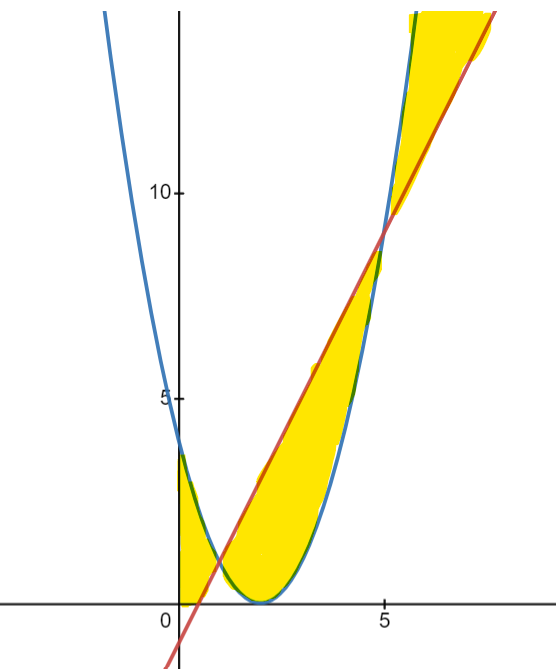
\includegraphics[width = 0.4\linewidth]{Images/area example .png}
\end{figure}
\paragraph{Answer} 
\begin{align*} 
    f(x) - g(x) &= x^2 - 4x + 4 - 2x + 1 \\
    &= x^2 - 6x + 5 \\
    &= (x - 5)(x - 1)
\end{align*}
\[
    \mid 0 \mid -- (+) -- \mid 1 \mid -- (-) -- \mid 5 \mid -- (+) -- \mid 8 \mid 
\]
\noindent
Hence,
\begin{align*} 
    A &= \int_0^{8} \mid f(x) - g(x) \mid\, dx \\
    &=  \int_0^{8} \mid x^2 - 6x + 5 \mid\: dx \\
    &= \int_0^{1} x^2 - 6x + 5 \mid\: dx - \int_1^{5} x^2 - 6x + 5 \mid\: dx + \int_5^{8} x^2 - 6x + 5 \mid\: dx \\
    &= 40
\end{align*}

\paragraph{Remark} Area $A$ between curves $x = f(y)$ and $x = g(y)$, from $y = a$ to $y = b$ can be defined similarly:
\[
    A = \int_a^b \mid f(y) - g(y) \mid\: dy
\]

\section{Substitution Method}
\begin{theorem}[The Substitution Rule]
    If $u = g(x)$ is a differentiable function whose range is an interval $I$, and $f$ is continuous on $I$, Then
    \[
        \int f(g(x))g'(x)\: dx= \int f(u)\: du
    \]
\end{theorem}
\paragraph{Proof}
Since $f$ is continuous, by FTC1 it has an antiderivative $F$. Let $f(x) = F'(x)$
\begin{align*} 
    \int f(g(x))g'(x)\: dx &= \int F'(g(x)) g'(x)\: dx \\
    &= \int (F \circ g)'(x)\: dx \\
    &= (F \circ g)(x) + C \\
    &= F(g(x)) + C \\
    &= F(u) + C \\
    &= \int F'(u) du = \int f(u) du
\end{align*}

\paragraph{Example 1} What is the antiderivative of $f(x) = \frac{1}{\sqrt{x}} \cos{\sqrt{x}}\: dx$?
\paragraph{Answer} Let $u = \sqrt{x}$, $du/dx = 1/2\sqrt{x}$.
\[
    \int \frac{1}{\sqrt{x}} \cos{\sqrt{x}}\: dx = \int 2 \cos{u}\: du = 2 \sin{u} + C = 2 \sin{\sqrt{x}} + C
\] 
Hence, $F(x) = 2 \sin{\sqrt{x}}$

\paragraph{Example 2} Find $\int \sin^3 x\: dx$ \\
Let $u = \cos x$, $dx = \frac{-1}{\sin x} du$
\begin{align*} 
    \int \sin^3 x\: dx &= \int (1 - \cos^2 x)\sin x\: dx \\
    &= \int (1 - \cos^2 x)\sin x\: dx \\
    &= \int -(1 - u^2)\; du \\
    &= \frac{1}{3} u^3 - u + C = \frac{1}{3} \cos^3 (x) - \cos (x) + C
\end{align*}
or, we may write $d(g(x))$ instead of $du$ if $u = g(x)$
\begin{align*} 
    \int \sin^3 x\: dx &= \int (1 - \cos^2 x)\sin x\: dx \\
    &= \int (1 - \cos^2 x)\sin x\: dx \\
    &= \int (\cos^2 - 1)( - \sin x)dx\\
    &= \int (\cos^2 - 1) d(\cos x)\\
    &= \frac{1}{3} \cos^3 (x) - \cos (x) + C
\end{align*}
\paragraph{Example 3} Find $\int x \sqrt{2x + 1}\: dx$ \\
Let $u = 2x + 1 \Rightarrow x = 1/2 (u - 1)$. Then $\frac{du}{dx} = 2 \Rightarrow dx = 1/2 du$
\begin{align*} 
    \int x \sqrt{2x + 1}\: dx &= \int \frac{u - 1}{2} \sqrt{u}\: \frac{1}{2}dx \\
    &= \frac{1}{4} \int u\sqrt{u} - \sqrt{u}\: du \\
    &= \frac{1}{4} (\frac{2}{5} u^ \frac{5}{2}) - \frac{2}{3}u^{\frac{3}{2}}) + C \\
    &= \frac{1}{4} (\frac{2}{5} (2x + 1)^ \frac{5}{2}) - \frac{2}{3}(@x + 1)^{\frac{3}{2}}) + C
\end{align*}

\paragraph{Remark} If $f$ is continuous on an interval $I$ and $F' = f$ on $I$, then
\[
    \int f(Ax + B)\: dx = \int f(u) \frac{1}{A}\: du = \frac{1}{A} F(u) + C = \frac{1}{A} F(Ax + B) + C
\]
\paragraph{Example} $\int \sec^2 (5x + 1)\: dx$ = $\frac{1}{5} \tan (5x + 1) + C$

\begin{theorem}[Substitution in Definite Integrals]
     If $g'$ is continuous on the interval $[a, b]$ and $f$ is continuous on the range of $g(x) = u$, then 
     \[
         \int_a^b f(g(x))\cdot g'(x)\: dx = \int_{g(a)}^{g(b)} f(u)\: du
     \]
\end{theorem}

\paragraph{Proof}
Let $F$ be an antiderivative of $f$ on range($g$). Then 
\begin{align*} 
     \int_{g(a)}^{g(b)} f(u)\: du &= F(g(b)) - F(g(a)) \\
     &= (F \circ g)(b) - (F \circ g)(a) \\
     &= \int_{a}^{b} (F \circ g)'(x)\: dx \\
     &= \int_{a}^{b} F'(g(x))g'(x)\: dx
\end{align*}
\paragraph{Example} $I = \int_{-1}^{1} 3x^2 \sqrt{x^2 + 1}\: dx$. Find $I$
\paragraph{Method 1} Let $u = x^3 + 1$, $du = 3x^2 dx$. $x = -1 \Rightarrow u = 0$ and $x = 1 \Rightarrow u = 2$
\[
    \int_{x = - 1}^{x = 1} 3x^2 \sqrt{x^3 + 1}\: dx = \int_{u = 0}^{u = 2} \sqrt{u}\: du = \frac{4}{3} \sqrt{2}
\]
\paragraph{Method 2} Find the antiderivative first:
\[
    \int 3x^2 \sqrt{x^3 + 1}\: dx = \int \sqrt{x^3 + 1}\: d(x^3 + 1) = \frac{2}{3} (x^3 + 1)^{\frac{3}{2}} + C
\]
Apply FTC2:
\[
    \int_{x = - 1}^{x = 1} 3x^2 \sqrt{x^3 + 1}\: dx = \left[\frac{2}{3} (x^3 + 1)^{\frac{3}{2}}\right]^{1}_{ - 1} = \frac{2}{3} \left(\sqrt{8} - 0\right) = \frac{4}{3} \sqrt{2}
\]
\section{Even and Odd Function}
\paragraph{Definition}
A function $f : D \to \mathbb{R}$ is called
\begin{itemize} 
    \item an even function, if $f(x) = f(-x)$ for all $x \in D$
    \item an odd function, if $f(x) = -f(-x)$ for all $x \in D$
\end{itemize}

\begin{theorem}[Integrals of Symmetric Functions]
     Let $f : [-a, a] \to \mathbb{R}$ be an integrable function
     \begin{itemize} 
        \item if $f$ is an even function, then $\int_{-a}^{a} f(x)\: dx = 2 \int_0^a f(x)\: dx$
        \item if $f$ is an odd function,  $\int_{-a}^{a} f(x)\: dx = 0$
    \end{itemize}
\end{theorem}
\paragraph{Proof}
If $f$ is even, then 
\begin{align*} 
    \int_{ - a}^{a} f(x)\: dx &= \int_{ - a}^0 f(x)\: dx + \int_0^a f(x)\: dx \\
    &= - \int_{0}^{ - a} f(x)\: dx + \int_0^a f(x)\: dx 
\end{align*}

Let $u = -x$, $dx = -du$
\begin{align*} 
    - \int_{0}^{ - a} f(x)\: dx + \int_0^a f(x)\: dx  &= - \int_{0}^{a} f( - u)\: - du + \int_0^a f(x)\: dx \\
    &= \int_{0}^{a} f( -u)\: du + \int_0^a f(x)\: dx  \\
    &= \int_{0}^{a} f(u)\: du + \int_0^a f(x)\: dx  \textrm{\tab since } f(-u) = f(u)\\
    &= 2\int_0^a f(x)\: dx\, 
\end{align*}

If $f$ is odd, then 
\begin{align*} 
    \int_{ - a}^{a} f(x)\: dx &= \int_{ - a}^0 f(x)\: dx + \int_0^a f(x)\: dx \\
    &= - \int_{0}^{ - a} f(x)\: dx + \int_0^a f(x)\: dx 
\end{align*}

Let $u = -x$, $dx = -du$
\begin{align*} 
    - \int_{0}^{ - a} f(x)\: dx + \int_0^a f(x)\: dx  &= - \int_{0}^{a} f( - u)\: - du + \int_0^a f(x)\: dx \\
    &= \int_{0}^{a} f( -u)\: du + \int_0^a f(x)\: dx  \\
    &= - \int_{0}^{a} f(u)\: du + \int_0^a f(x)\: dx  \textrm{\tab since } f(-u) = -f(u)\\
    &= 0 
\end{align*}

\paragraph{Example 1} Show that $I = \int_{-\sqrt{2}}^{\sqrt{2}} (15x^4 - 4x^3 + 6x^2 + 7x)\: dx = 32 \sqrt{2}$
\[
    I = \int_{-\sqrt{2}}^{\sqrt{2}} (15x^4 + 6x^2)\: dx + \int_{-\sqrt{2}}^{\sqrt{2}} ( - 4x^3 + 7x)\: dx
\]
Since $15x^4 + 6x^2$ is an even function and $ - 4x^3 + 7x$ is an odd function, then
\[
    I = 2 \int_{0}^{\sqrt{2}} (15x^4 + 6x^2)\: dx = 32 \sqrt{2}
\]

\paragraph{Example 2} Show that $I = \int_{-1}^{3} (x + 1)^2(x - 3)^2\: dx = 512/15$ \\
First we will show that the function is symmetrical about $x = 1$
\begin{align*} 
    f(x_0 + \delta) &= f(x_0 - \delta) \textrm{\tab} \forall \delta > 0 \\
    (x_0 + \delta + 1)^2(x_0 + \delta - 3)^2 &= (x_0 - \delta + 1)^2(x_0 - \delta - 3)^2 \\
\end{align*}
Let $\delta  = 1$
\begin{align*} 
    (x_0 + 2)^2(x_0 - 2)^2 &= (x_0)^2(x_0 - 4)^2 \\
    x_0 &= 1
\end{align*}
\noindent
Let $u = x - 1$, then $du = dx$
\begin{align*} 
    I &= \int_{ - 2}^{2} (u + 2)^2(u - 2)^2\: du \\
    &= \int_{ - 2}^{2} ((u + 2)(u - 2))^2 \: du \\
    &= \int_{ - 2}^{2} (u^2 - 4)^2 \: du \\
    &= \int_{ - 2}^{2} (u^4 - 8u^2 + 16) \: du \\
    &= 2 \int_{0}^{2} (u^4 - 8u^2 + 16) \: du \\
    &= 2 \left[ \frac{1}{5}u^5 - \frac{8}{3}u^3 + 16u \right]^2_0 = \frac{512}{15}
\end{align*}
\end{document}
